\documentclass[article]{jss}
\usepackage[utf8]{inputenc}

\providecommand{\tightlist}{%
  \setlength{\itemsep}{0pt}\setlength{\parskip}{0pt}}

\author{
Pedro Albuquerque\\University of Brasilia \And Denis Ribeiro do Valle\\University of Florida \And Daijiang Li\\University of Florida
}
\title{Bayesian LDA for categorical mixture model clustering.}
\Keywords{LDA, fuzzy clustering, categorical data, pattern recognition}

\Abstract{
The goal of this paper is to describe the Bayesian LDA model for fuzzy
clustering based on different types of data (i.e., Multinomial,
Bernoulli, and Binomial entries), provide some examples of the use of
this model in R, and to introduce a new R package called Rlda. These
types of data frequently emerge in fields as disparate as ecology,
remote sensing, marketing, and finance. As result, we believe this
package will be of broad interest for pattern recognition, particularly
fuzzy clustering for categorical data.
}

\Plainauthor{Pedro Albuquerque, Denis Ribeiro do Valle, Daijiang Li}
\Plaintitle{Bayesian LDA for categorical mixture model clustering.}
\Shorttitle{\pkg{Rlda}: Bayesian LDA for categorical clustering.}
\Plainkeywords{LDA, fuzzy clustering, categorical data, pattern recognition}

%% publication information
%% \Volume{50}
%% \Issue{9}
%% \Month{June}
%% \Year{2012}
\Submitdate{}
%% \Acceptdate{2012-06-04}

\Address{
    Pedro Albuquerque\\
  University of Brasilia\\
  Faculdade de Economia, Administracao e Contabilidade, Building A-2 -
  Office A1-54/7, Brasilia, DF 70910-900.\\
  E-mail: \href{mailto:pedroa@unb.br}{\nolinkurl{pedroa@unb.br}}\\
  URL: \url{http://pedrounb.blogspot.com/}\\~\\
      Denis Ribeiro do Valle\\
  University of Florida\\
  408 McCarty Hall C, PO Box 110339, Gainesville, FL 32611-0410.\\
  E-mail: \href{mailto:drvalle@ufl.edu}{\nolinkurl{drvalle@ufl.edu}}\\
  URL: \url{http://denisvalle.weebly.com/}\\~\\
      Daijiang Li\\
  University of Florida\\
  408 McCarty Hall C, PO Box 110339, Gainesville, FL 32611-0410.\\
  E-mail: \href{mailto:daijianglee@gmail.com}{\nolinkurl{daijianglee@gmail.com}}\\
  URL: \url{http://daijiang.name/}\\~\\
  }

\usepackage{amsmath} \usepackage{amsfonts} \usepackage{bbm}
\usepackage{calrsfs} \usepackage{draftwatermark} \usepackage{graphicx}
\usepackage{wrapfig} \usepackage{lscape} \usepackage{rotating}
\usepackage{epstopdf} \SetWatermarkText{DRAFT} \SetWatermarkScale{1}
\newcommand{\Za}{\mathcal{Z}}

\begin{document}

\section{Introduction.}\label{introduction.}

The Latent Dirichlet Allocation model (LDA), first proposed by Blei, Ng,
and Jordan (2003), has been extensively used for text-mining in multiple
fields. Tsai (2011) used LDA to construct clusters of tags that
represent the most common topics in blogs. Lee et al. (2010) compared
LDA against three other text mining methods that are frequently used:
latent semantic analysis, probabilistic latent semantic analysis, and
the correlated topic model. The limitations of LDA, as identified by
these authors, were that the method does not consider relationship
between topics and cannot allocate a given word to multiple topics
simultaneously as a fuzzy clustering approach does. Despite these
limitations, however, LDA continues to be used in multiple disciplines.
For instance, Griffiths and Steyvers (2004) used LDA to identify the
main scientific topics in a large corpus of the Proceedings of the
National Academy of Science articles. In conservation biology, LDA has
been used to identify research gaps in the conservation literature
(Westgate et al. 2015). LDA has also been proposed as a promising method
for the automatic annotation of remote sensing imagery (Lienou, Maître,
and Datcu 2010). In marketing, LDA has been used to extract information
from product reviews across 15 firms in five markets over four years,
enabling the identification of the most important latent dimensions of
consumer decision making in each studied market (Tirunillai and Tellis
2014). Finally, in finance, a stock market analysis system based on LDA
was used to combine financial news items together with stock market data
to identify and characterize major events that impact the market. This
system was then used to make predictions regarding stock market
behaviour based on news items identified by LDA (Mahajan, Dey, and Haque
2008).

Despite its success in text mining across multiple fields, LDA is a
model that need not be restricted to text-mining. More specifically, LDA
can be viewed as a mixture model since each element in the sample can
belong to more than one cluster (or state) simultaneously. There are a
few examples of LDA being used for other purposes than text-mining. For
instance, a modified version of LDA has been extensively used on genetic
data to identify populations and admixture probabilities of individuals
(Pritchard, Stephens, and Donnelly 2000). Similarly, LDA has been used
in ecology to identify plant communities from tree data for the eastern
United States and from a tropical forest chronosequence (Valle et al.
2014).

The aim of this paper is to describe a Bayesian LDA model for mixture
model clustering based on different types of data (i.e., multinomial,
Bernoulli and Binomial), illustrating its use in a diverse set of
examples. The innovative features of this model are that it generalizes
LDA for other types of commonly encountered categorical data and it
enables the selection of the optimal number of clusters based on a
truncated stick-breaking prior approach which regularizes model results.
Finally, we provide a package to fit this novel Bayesian LDA model.

This paper is organized as follows. Section 2 describes the mathematical
formulation for the Bayesian LDA model and section 3 shows how the model
was implemented in R. Sections 4 and 5 present examples of the use of
the package and the conclusions, respectively.

\section{Methods.}\label{methods.}

In the Bayesian LDA model for fuzzy clustering we postulate that each
element is allocated to a single cluster, represented by a latent state
variable. Specifically, consider a latent matrix \(\mathbf{Z}\) with
dimension equals to \(L\times C\) where each row represents a sampling
unit (\(l=1,\dots,L\)) and each column a possible state or cluster
(\(c=1,\dots,C\)). The Data Generating Process postulated for this
latent matrix is given by:

\begin{equation}
\boldsymbol Z_{l\cdot}\sim Multinomial(n_{l},\boldsymbol\theta_{l})
\label{eq:eq0001}
\end{equation}

\noindent where \(n_{l}\) is total number of elements drawn for location
\(l\) and \(\boldsymbol\theta_{l}=(\theta_{l1},\dots,\theta_{lC})\) is a
vector of parameters representing the probability of allocation in each
cluster. Following Occam's razor, we intend to create the least number
of clusters as possible, which is achieved by assuming a truncated
stick-breaking prior:

\begin{equation}
\theta_{lc}=V_{lc}\displaystyle\prod_{c^{*}=1}^{c-1}(1-V_{lc^{*}})
\label{eq:eq0002}
\end{equation}

\noindent where \(V_{lc}\sim Beta(1,\gamma)\) for \(c=1,\dots,C-1\) and
\(V_{lC}=1\) by definition. This truncated stick-breaking prior will
force the elements to be aggregated in the minimum number of clusters,
given that \(\theta_{lc^{*}}\) is stochastically exponentially
decreasing.

In the second hierarchical level, we consider a matrix \(\mathbf{Y}\)
with dimension equal to \(L\times S\) where each row represents a
sampling unit (e.g., locations, firms, individuals, plots) and each
column a variable that describes these elements. In the Bayesian LDA
model for fuzzy clustering, after integrating over the latent vector
\(\mathbf{Z}_{l\cdot}\), \(Y_{ls}\) can follow one of these
distributions:

\begin{equation}
\begin{cases}
\mathbf{Y}_{l\cdot}\sim Multinomial(n_{l},\boldsymbol\theta_{i}^{t}\Phi)\\
Y_{ls}\sim Bernoulli(\boldsymbol\theta_{i}^{t}\boldsymbol\phi_{s})\\
Y_{ls}\sim Binomial(n_{ls},\boldsymbol\theta_{i}^{t}\boldsymbol\phi_{s})
        \label{eq:eq0003}
\end{cases}     
\end{equation}

\noindent for \(l=1,\dots,L\) and \(s=1,\dots,S\) possible variables.
\(Y_{ls}\) represents a random variable, \(\boldsymbol Y_{l\cdot}\) is a
vector with these random variables for location \(l\), \(n_{l}\) is the
total number of elements in sampling unit \(l\), \(n_{ls}\) is the total
number of elements in sampling unit \(l\) and variable \(s\). In these
models, \(\boldsymbol\phi_{s}=(\phi_{1s},\dots,\phi_{Cs})\) is a vector
of parameters, while \(\boldsymbol\Phi\) is a \(C\times S\) matrix of
parameters, given by:

\[
\mathbf{\Phi}=\begin{bmatrix}
    \phi_{11} & \phi_{12} & \dots  & \phi_{1S} \\
    \phi_{21} & \phi_{22} & \dots  & \phi_{2S} \\
    \vdots & \vdots  & \ddots & \vdots \\
    \phi_{C1} & \phi_{C2} & \dots  & \phi_{CS} 
\end{bmatrix}
\]

In the last step, we specify the priors for \(\phi_{cs}\). For the
multinomial model, we adopt a Dirichlet prior (i.e.
\(\boldsymbol\phi_{c}\sim Dirichlet(\boldsymbol\beta)\) where
\(\boldsymbol\beta=(\beta_{1},\dots,\beta_{S})\) is the hyperparameter
vector). For the Bernoulli and Binomial representations, we assume that
\(\phi_{cs}\) comes from a Beta distribution, (i.e.,
\(\phi_{cs}\sim Beta(\alpha_{0},\alpha_{1})\)).

These models are fit using Gibbs Sampling where parameter draws are
iteratively made from each full conditional distribution. From a
conceptual perspective, all of these models assume the following matrix
decomposition:

\begin{equation}
\mathbb{E}[\mathbf{Y}_{L\times S}]=\mathbf{K}\circ[\Theta_{L\times C}\Phi_{C\times S}]
    \label{eq:eq0004} 
\end{equation}

where \(\mathbf{K}\) is a matrix of constants and \(\circ\) is the
Hadamard product. Sparseness is ensured by forcing large \(c\) in the
\(\Theta_{L\times C}\) matrix to be close to zero. For the multinomial
model, the \(\mathbf{K}\) matrix contains the total number of elements
in each row whereas for the Bernoulli model, this matrix is equal to the
identity matrix. Finally, for the Binomial model, the \(\mathbf{K}\)
matrix has the total number of trials of each binomial distribution
(i.e., \(n_{ls}\)). Although there are many ways matrices can be
decomposed, the key characteristic of this particular form of matrix
decomposition is that each row of \(\mathbf{\Theta}\) is comprised of
probabilities that sum to one. As a result, one can interpret
\(\Phi_{C\times S}\) as the matrix that contain the ``pure'' features of
the data, which are then mixed by the matrix \(\Theta_{L\times C}\) and
multiplied by \(\mathbf{K}\) to generate the expected data.

\subsection{Full Conditional Distributions -
FCD.}\label{full-conditional-distributions---fcd.}

\subsubsection{Bernoulli model.}\label{bernoulli-model.}

The probability of community membership status \(Z_{ls}\) is given by:

\begin{equation}
\begin{array}{lll}
p(Z_{ls}=c^{*}|...)&=&\frac{\theta_{lc^{*}}\phi_{c^{*}s}^{y_{ls}}(1-\phi_{c^{*}s})^{1-y_{ls}}}{\displaystyle\sum_{c=1}^{C}\theta_{lc}\phi_{cs}^{y_{ls}}(1-\phi_{cs})^{1-y_{ls}}}
\end{array}
\label{eq:eq0005} 
\end{equation}

Therefore, \(Z_{ls}\) can be drawn from a categorical distribution. The
FCD for \(V_{lc}\) is given by:

\[
p(V_{lc}|...)=Beta(N_{lc}+1,N_{l(c^{*}>c)}+\gamma)
\]

\noindent where \(N_{lc}\) is the total number of elements in location
\(l\) classified into cluster \(c\), and \(N_{l(c^{*}>c)}\) is the total
number of elements in location \(l\) classified in clusters larger than
\(c\). These quantities are given by
\(N_{lc}=\sum_{s=1}^{S}\mathbbm{1}(z_{ls}=c)\) and
\(N_{l(c^{*}>c)}=\sum_{s=1}^{S}\sum_{c^{*}=c+1}^{C}\mathbbm{1}(z_{ls}=c^{*})\),
respectively. Finally, the FCD for \(\phi_{cs}\) is given by:

\[
p(\phi_{cs}|...)=Beta(N_{cs}^{(1)}+\alpha_0,N_{cs}^{(0)}+\alpha_1)
\]

\noindent where \(N_{cs}^{(1)}\) is the number of elements assigned to
cluster \(c\) and for which \(Y_{ls}=1\) (i.e.,
\(\sum_{l=1}^L\mathbbm{1}(z_{ls}=c,Y_{ls}=1)\)) and \(N_{cs}^{(0)}\) is
the number of elements assined to cluster \(c\) and for which
\(Y_{ls}=0\) (i.e., \(\sum_{l=1}^L\mathbbm{1}(z_{ls}=c,Y_{ls}=0)\)).

\subsubsection{Binomial model.}\label{binomial-model.}

For this model, we have \(n_{ls}\) elements for each sampling unit \(l\)
and community \(z\). The \(i\)-th element is denoted as \(Z_{ils}\) and
its probability is similar to the one for the Bernoulli model:

\begin{equation}
\begin{array}{lll}
p(Z_{lc}=c^{*}|...)&=&\frac{\theta_{lc^{*}}\phi_{c^{*}s}^{x_{ils}}(1-\phi_{c^{*}s})^{1-x_{ils}}}{\displaystyle\sum_{c=1}^{C}\theta_{lc}\phi_{cs}^{x_{ils}}(1-\phi_{cs})^{1-x_{ils}}}
\end{array}
\label{eq:eq0006} 
\end{equation}

\noindent where \(x_{ils}\) are binary random variables such that
\(\sum_{i=1}^{n_{ls}}x_{ils}=y_{ls}\). Therefore, \(Z_{ils}\) can be
drawn from a multinomial distribution. The FCD for \(\phi_{cs}\) is
given by:

\begin{equation}
\begin{array}{lll}
p(\phi_{cs}|...)= Beta\left(\displaystyle\sum_{l=1}^{L}\displaystyle\sum_{i=1}^{n_{ls}}\mathbbm{1}(x_{ils}=1,z_{ils}=c)+\alpha_{0},\displaystyle\sum_{l=1}^{L}\displaystyle\sum_{i=1}^{n_{ls}}\mathbbm{1}(x_{ils}=0,z_{ils}=c)+\alpha_{1}\right)
\end{array}
\label{eq:eq0007} 
\end{equation}

Finally, the FCD for \(V_{lc}\) is given by:

\begin{equation}
p\left(V_{lc}|...\right) = Beta(N_{lc}+1,N_{l(c^{*}>c)}+\gamma)
    \label{eq:eq0008} 
\end{equation}

\noindent where \(N_{lc}\) is the total number of elements in location
\(l\) classified into cluster \(c\) and \(N_{l(c^{*}>c)}\) is the total
number of elements in location \(l\) classified in clusters larger than
\(c\). These quantities are given by
\(N_{lc}=\sum_{s=1}^{S}\sum_{i=1}^{n_{ls}}\mathbbm{1}(z_{ils}=c)\) and
\(N_{l(c^{*}>c)}=\sum_{s=1}^{S}\sum_{i=1}^{n_{ls}}\sum_{c^{*}=c+1}^{C}\mathbbm{1}(z_{ils}=c^{*})\).

\subsubsection{Multinomial model.}\label{multinomial-model.}

For the Multinomial case, if unit \(i\) in location \(l\) is associated
with variable \(s\) (i.e., \(x_{il}=s\) such that
\(y_{ls}=\sum_{i=1}^{n_{l}}\mathbbm{1}(x_{il}=s)\)), we have that:

\begin{equation}
p(Z_{il}=c^{*}|...)=\frac{\theta_{lc^{*}}\phi_{sc^{*}}}{\left(\theta_{1l}\phi_{s1}+\dots+\theta_{Cl}\phi_{sC}\right)}
    \label{eq:eq0009} 
\end{equation}

Therefore, \(Z_{il}\) can be sampled from a categorical distribution.
Since we assumed a conjugate prior for \(\boldsymbol\phi_{c^{*}}\) with
\(c^{*}\in\{1,\dots,C\}\) the Full Conditional Distribution for this
vector of parameters is a straight-forward Dirichlet distribution:

\begin{equation}
p(\boldsymbol\phi_{c^{*}}|...)=Dirichlet([n_{c^{*}1}+\beta_{1},\dots,n_{c^{*}S}+\beta_{S}])
    \label{eq:eq0010} 
\end{equation}

\noindent where \(n_{c^{*}s}\) is the total number of observations
classified in cluster \(c^{*}\) in all locations for the \(s\)-th
variable (i.e.,
\(n_{c^{*}s}=\sum_{l=1}^{L}\sum_{i=1}^{n_{l}}\mathbbm{1}(z_{il}=c^{*},x_{il}=s)\)).

Finally, the FCD for \(V_{lc^{*}}\) is given by:

\begin{equation}
  p(V_{lc^{*}}|...)=Beta(N_{lc^{*}}+1,N_{l(c>c^{*})} +\gamma)
    \label{eq:eq0011} 
\end{equation}

\noindent where \(N_{lc^{*}}\) is the total number of elements in
observation \(l\) classified into cluster \(c^{*}\) and
\(N_{l(c>c^{*})}\) is the total number of elements in observation \(l\)
classified in clusters larger than \(c^{*}\). These quantities are given
by \(N_{lc^{*}}=\sum_{i=1}^{n_{l}}\mathbbm{1}(z_{il}=c^{*})\) and
\(N_{l(c>c^{*})}=\sum_{i=1}^{n_{l}}\sum_{c=c^{*}+1}^{C}\mathbbm{1}(z_{il}=c)\).

\section{The Rlda package.}\label{the-rlda-package.}

We found four other packages that can fit the Latent Dirichlet
Allocation model. Hornik and Grün (2011) developed the \pkg{topicmodels}
package for which there are two LDA implementations, one using the
variational inference (as described in Blei, Ng, and Jordan (2003)) and
the other implementation using Gibbs Sampling based on Phan and Nguyen
(2013). Similarly, Jones (2016) proposed the \pkg{textmineR} which
relies on Gibbs Sampling to estimate the topics in a corpus structure.
Chang (2012) developed the \pkg{lda} package which includes the
mixed-membership stochastic blockmodel (Airoldi et al. 2008), supervised
Latent Dirichlet Allocation - sLDA (Mcauliffe and Blei 2008) and
Correspondence-Latent Dirichlet Allocation - corrLDA(Blei and Jordan
2003). Finally, more recently, Roberts, Stewart, and Tingley (2014)
created the \pkg{stm} which has some unsupervised functions to determine
the optimal number of clusters. This unsupervised method is based on
likelihood metrics obtained by the EM Algorithm, which are then used
within a backward model selection approach.

None of these packages adopt the truncated stick-breaking prior which
enables the selection of the optimal number of clusters and regularizes
model results. Furthermore, none of them use others distributions
besides the Multinomial outcome for the dependent variable. Thus, our
Rlda package complements current LDA approaches already available in R.

\section{Examples.}\label{examples.}

In this section we present some applications for Latent Dirichlet
Allocation in marketing, remote sensing and ecology.

\subsection{Marketing.}\label{marketing.}

The first application considers the classical LDA for a Multinomial
entry in the field of Marketing. More specifically, we are interested in
characterizing firms based on their consumers' complaints.

It is well known that attracting a new customer is often considerably
costlier than keeping current customer (Kotler and Armstrong 2006). For
this reason, firms can better retain their customers if they pay careful
attention to their consumers' complaints and work to solve them in a
satisfactory way.

The data come from the 2015
\href{http://catalog.data.gov/dataset/consumer-complaint-database}{Consumer
Complaint Database} and consist of complaints received by the
\textbf{Bureau of Consumer Financial Protection} in US regarding
financial products and services. In this example, we work only with
credit card complaints. This dataset contains information on the number
of complaints for each firm (\(L=\) 226), categorized according to the
specific type of issue (\(S=\) 30). Examples of issues include billing
disputes, identity theft / fraud, and unsolicited issuance of credit
card. Each sampling unit in this case represents a firm and each
variable the total number of complaints associated with each issue.

The characterization of firms provided by our analysis can be useful to
reveal communalities and differences across different firms. This can
then be used by managers to identify and potentially adopt the solutions
that are employed by other firms to deal with these issues.

To use the \pkg{Rlda} package for the Multinomial entry is necessary to
create a matrix where each cell represents the total number of cases
observed for each variable and sampling unit.

\begin{CodeChunk}
\begin{CodeInput}
library(Rlda)
#Read the Complaints data
data(complaints)
#Create the abundance matrix
library(reshape2)
mat1<-dcast(complaints[,c("Company","Issue")], 
            Company~Issue, length, 
            value.var="Issue")
#Create the rowname
rownames(mat1)<-mat1[,1]
#Remove the ID variable
mat1<-mat1[,-1]
\end{CodeInput}
\end{CodeChunk}

To use the \code{lda_multinomial} method we need to specify some
arguments:

\begin{CodeChunk}
\begin{CodeInput}
#Set seed
set.seed(9292)
#Hyperparameters for each prior distribution
beta<-rep(1,ncol(mat1))
gamma<-0.01
#Execute the LDA for the Multinomial entry
res<-lda_multinomial(data=mat1,n_community=30,beta,gamma,n_gibbs=1000,
                     ll_prior=TRUE,display_progress=FALSE)
\end{CodeInput}
\end{CodeChunk}

In the above code we set the maximum number of clusters to 30 and the
number of Gibbs Sampling iterations to 1000. Furthermore, we ask that
the algorithm output the sum of the log-likelihood and the log-prior.
Finally, we chose not to display the progress bar.

We can visually evaluate the convergence by examining Figure
\ref{figure:fig001}:

\begin{CodeChunk}
\begin{CodeInput}
#Get the logLikelihood
ll<-res[["logLikelihood"]]
#Plot the log-likelihood
plot(ll,type="l",xlab="Interations",
                 ylab="Log-likelihood")
\end{CodeInput}
\end{CodeChunk}

\begin{figure}[htbp]
  \centering
  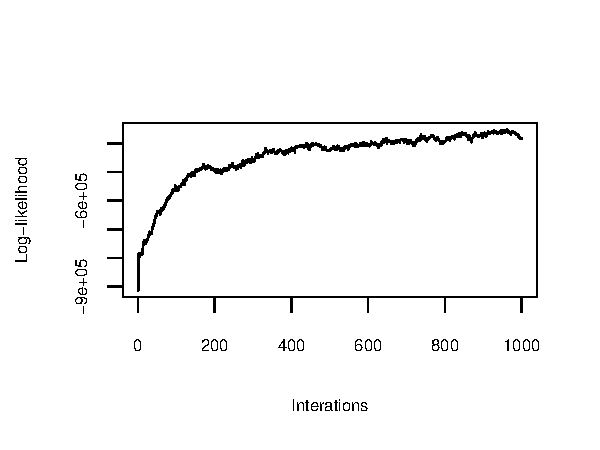
\includegraphics{plot001.pdf}
  \caption{Log-likelihood interations.}
  \label{figure:fig001}
\end{figure}

Samples of our parameter estimates are given in the \code{Theta} and
\code{Phi} matrices. Each line in these matrices contains the result of
a Gibbs iteration. This way, we can get parameter estimates based on the
columns of these matrices after discarding iterations prior to the
\emph{burn-in phase}.

\begin{CodeChunk}
\begin{CodeInput}
#Get the Theta Estimate
Theta<-res[["Theta"]]
#Burnout
Theta<-colMeans(Theta[300:1000,])
#Create the matrix
Theta<-matrix(Theta,nrow = nrow(mat1),ncol=30)
#Rownames
rownames(Theta)<-rownames(mat1)
\end{CodeInput}
\end{CodeChunk}

The \code{Theta} matrix has a sparse structure since our truncated
stick-breaking prior tends to reduce the total number of dominant
clusters. Each cell contains the estimated probability of the \(l\)-th
firm being allocated to cluster \(c\).

To describe each cluster, we can examine the \code{Phi} matrix:

\begin{CodeChunk}
\begin{CodeInput}
#Get the Phi Estimate
Phi<-res[["Phi"]]
#Burnout
Phi<-colMeans(Phi[300:1000,])
#Create the matrix
Phi<-matrix(Phi,nrow =30,ncol=ncol(mat1))
#Colnames
colnames(Phi)<-colnames(mat1)
#Rownames
rownames(Phi)<-paste0("Cluster ",seq(1,30))
#Get the most likely issues
ids<-which(Phi > 0.2, arr.ind = TRUE)
\end{CodeInput}
\end{CodeChunk}

The most likely issues in each cluster are summarized as follow:

\begin{table}[ht]
\centering
\begingroup\fontsize{9pt}{10pt}\selectfont
\begin{tabular}{rl}
  \hline
Cluster & Issue \\ 
  \hline
7 & Advertising and marketing \\ 
  7 & Rewards \\ 
  17 & Closing/Cancelling account \\ 
  26 & Unsolicited issuance of credit card \\ 
   \hline
\end{tabular}
\endgroup
\caption{Clusters description.} 
\end{table}

Based on that information we can now analyze the firms with the highest
probability to belong to these clusters:

\begin{table}[ht]
\centering
\begingroup\fontsize{9pt}{10pt}\selectfont
\begin{tabular}{llr}
  \hline
Firm & Cluster & Probability \\ 
  \hline
U.S. Bancorp & Cluster 7 & 0.5239 \\ 
  Amex & Cluster 7 & 0.1878 \\ 
  Barclays PLC & Cluster 7 & 0.0974 \\ 
  Discover & Cluster 7 & 0.0511 \\ 
  PayPal Holdings, Inc. & Cluster 7 & 0.0153 \\ 
  U.S. Bancorp & Cluster 17 & 0.0000 \\ 
  Amex & Cluster 17 & 0.0000 \\ 
  Barclays PLC & Cluster 17 & 0.0000 \\ 
  Discover & Cluster 17 & 0.2957 \\ 
  PayPal Holdings, Inc. & Cluster 17 & 0.0088 \\ 
  U.S. Bancorp & Cluster 26 & 0.0000 \\ 
  Amex & Cluster 26 & 0.0000 \\ 
  Barclays PLC & Cluster 26 & 0.0000 \\ 
  Discover & Cluster 26 & 0.0000 \\ 
  PayPal Holdings, Inc. & Cluster 26 & 0.3958 \\ 
   \hline
\end{tabular}
\endgroup
\caption{Probability of belonging for each company.} 
\end{table}

The results are consistent with the type of product studied, in this
case \emph{Credit card}. It is interesting to note that the Cluster 7 is
mostly represented by financial services corporation such as U.S.
Bancorp and Amex. This cluster is mostly represented by
\emph{Advertising and marketing} and \emph{Rewards} issues which may
represent a larger cluster of complaints, for instance \emph{Deceptive
advertising complaints}.

Managers of those companies can use this information to create, for
example, a specific department to solve this disputes and/or clarify
their consumers about the \emph{Advertising} and \emph{Rewards} rules
and conditions, aiming to avoid misunderstood about the programs.

Cluster 17 on the other hand is mostly represented by firms with
\emph{Closing/Cancelling account} complaints and its most representative
firm is Discover which is also a financial services corporation but,
differently of the firms with large participation in Cluster 7, this
firm has complaints about \emph{Closing/Cancelling account}. For these
companies that belong to Cluster 17 they could focus their attention in
provide easy steps to \emph{Closing/Cancelling account} in a way to
avoid more complaints and improve their Customer Relationship Management
(CRM).

The final cluster is represented by financial services corporation that
act in most part on web, and its representative firm is PayPal Holdings,
Inc. The most likely issue associated with these companies that belongs
to Cluster 26 is \emph{Unsolicited issuance of credit card}.

These results can be explained by a change in the PayPal operations. The
complaints are related with the type of account provided by PayPal which
were converted from standard PayPal account to a revolving credit
account and some consumers claims to be unaware of this change, and
again, a good communication system between the company and its consumers
could avoid and easily solve complaints about those issues.

\subsection{Remote Sensing.}\label{remote-sensing.}

Because pixels in remote sensing imagery are often large enough to
encompass different substances within each pixel, there has been great
interest in the development of methods that enable researchers to
estimate the proportion of the constituent materials. Indeed, numerous
spectral unmixing algorithms have already been developed in the
literature, with multiple approaches used for the dimension reduction,
endmember determination, and inversion stages (Keshava 2003).

The key characteristics of the method that we propose here is that it is
an unsupervised method (i.e., it does not require the a priori
determination of endmembers) that enforces parsimony through our
truncated stick-breaking prior. Differently from many of the currently
existing methods for spectral unmixing, our model explicitly
acknowledges the discreteness of the digital numbers used in remote
sensing systems and the range of possible values these numbers can take.

In our example, we rely on Landsat TM 5 imagery from 2010 of the
Iquitos-Nauta road in the Peruvian Amazon. This area has multiple
land-use land-cover (LULC) types and is the site in which we have
studied the effect of these different LULC types on the malaria vector
\emph{Anopheles darlingi} (Tucker-Lima, n.d.).

\begin{CodeChunk}
\begin{CodeInput}
library(Rlda)
data("Landsat")
#Define the hyperparameters
a.phi  <- 0.1
b.phi  <- 9.9
ngibbs <- 10000
#Execute the Binomial LDA
z <- lda_binomial(data= Landsat,pop= max2, n_community=5,
                  alpha0= a.phi,alpha1= b.phi,gamma= 1,n_gibbs= ngibbs,
                  ll_prior=TRUE,display_progress=FALSE)
\end{CodeInput}
\end{CodeChunk}

In a similar way as presented in the Marketing example, we can get the
\code{Phi} and \code{Theta} matrices:

\begin{CodeChunk}
\begin{CodeInput}
#Total number of gibbs simulations
ngibbs <- 10000
#Sequence
seq1 <- floor(seq(from=(2/3)*ngibbs,to=ngibbs,length.out=1000))
#Theta matrix
theta1 <- z$Theta[seq1,] 
#Phi matrix
phi1   <- z$Phi[seq1,]
\end{CodeInput}
\end{CodeChunk}

Using these data, it is possible to construct some predictions to the
Iquitos-Nauta road in the Peruvian Amazon for each cluster:

\begin{figure}[htbp]
  \centering
  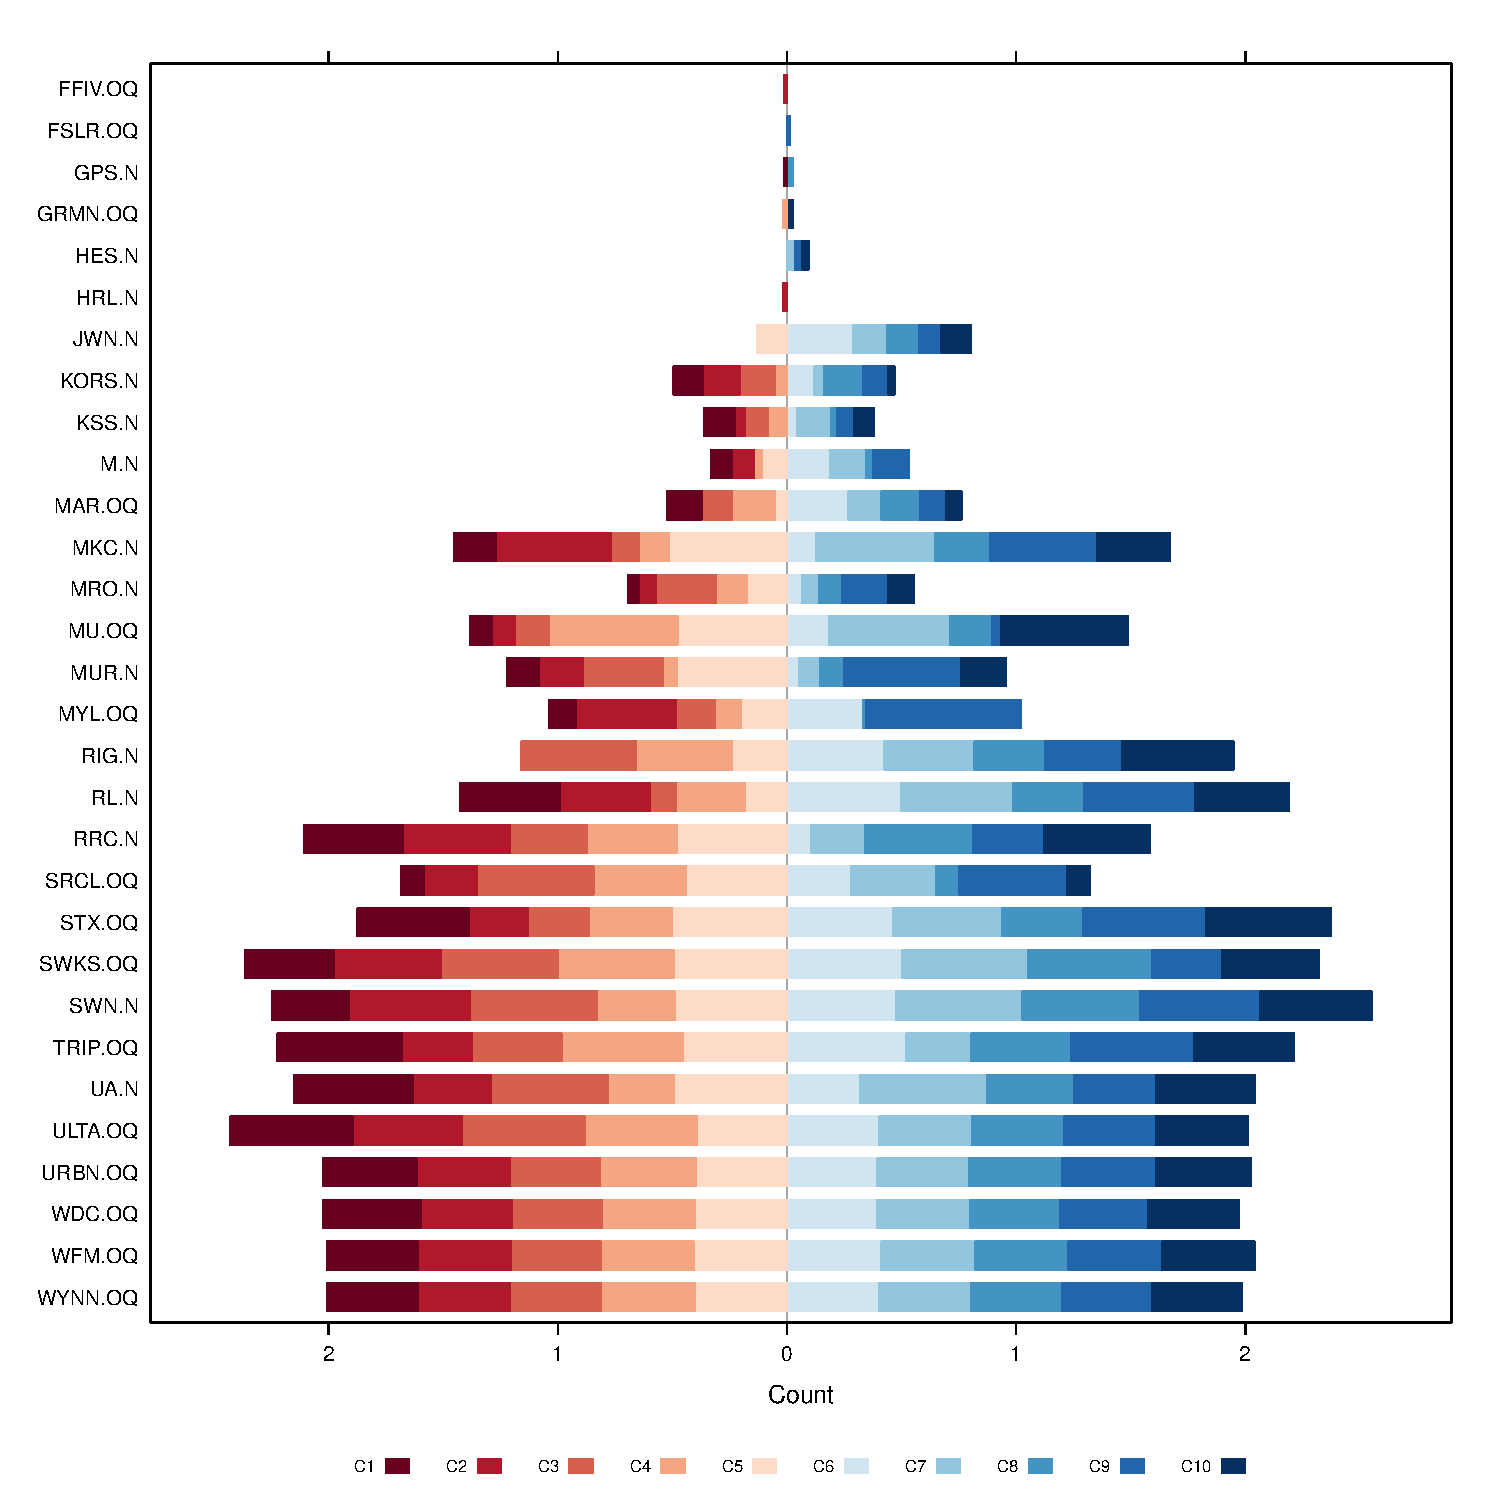
\includegraphics[width=17cm,height=12cm,keepaspectratio]{plot002.pdf}
  \caption{Clusters - Iquitos-Nauta road.}
  \label{figure:fig002}
\end{figure}

We can note different level of colors in the region which also vary
depending on the cluster chosen (the full high-resolution figures are
presented in the final of the paper). This similarity between regions is
due to the band's share and was modeled by the Binomial LDA. In other
words, some regions with red color represent regions whose can be
similar with respect to the LDA results and can represent villages,
streets, etc. For example, it is easy to see in Cluster 5 the roads and
deforested areas looking the pattern presented. Hence, the method can be
used to classify regions in an unsupervised way to solve pixel unmixing
problems.

\subsection{Ecology.}\label{ecology.}

In many ecological studies, it is not possible to determine the total
number of individuals per species in each sampling unit. As a result,
these data are often summarized into binary presence/absence matrices (1
and 0, respectively) (Pearce and Boyce 2006).

In this example we used \code{data("SPDATA")} from \pkg{PresenceAbsence}
package, which includes presence/absence information on 13 species at
386 forested locations (Moisen et al. 2006). We analyze these data using
the \code{lda_bernoulli} function.

\begin{CodeChunk}
\begin{CodeInput}
library(PresenceAbsence)
#Read SPDATA data
data(SPDATA)
PresAbs<-SPDATA[,1:2]
#Location
library(data.table)
PresAbs <- data.table(PresAbs)
PresAbs[, Location := sequence(.N), by = c("SPECIES")]
#Create the binary matrix
library(reshape2)
mat1<-dcast(PresAbs, 
            Location~SPECIES,  
            value.var="OBSERVED")
#Remove the Location variable
matPres<-as.data.frame(mat1[,-1])
\end{CodeInput}
\end{CodeChunk}

We use the following arguments for the \code{lda_bernoulli} function:

\begin{CodeChunk}
\begin{CodeInput}
#Set seed
set.seed(9842)
#Hyperparameters for each prior distribution
gamma <-0.01
alpha0<-0.01
alpha1<-0.01
#Execute the LDA for the Binomial entry
res<-lda_bernoulli(matPres,10,
                           alpha0,alpha1,gamma,
                           5000,TRUE,FALSE)
\end{CodeInput}
\end{CodeChunk}

We can visually evaluate the cluster distribution across species, after
the \emph{burn-in phase} in Figure \ref{figure:fig003}:

\newpage

\begin{figure}[htbp]
  \centering
  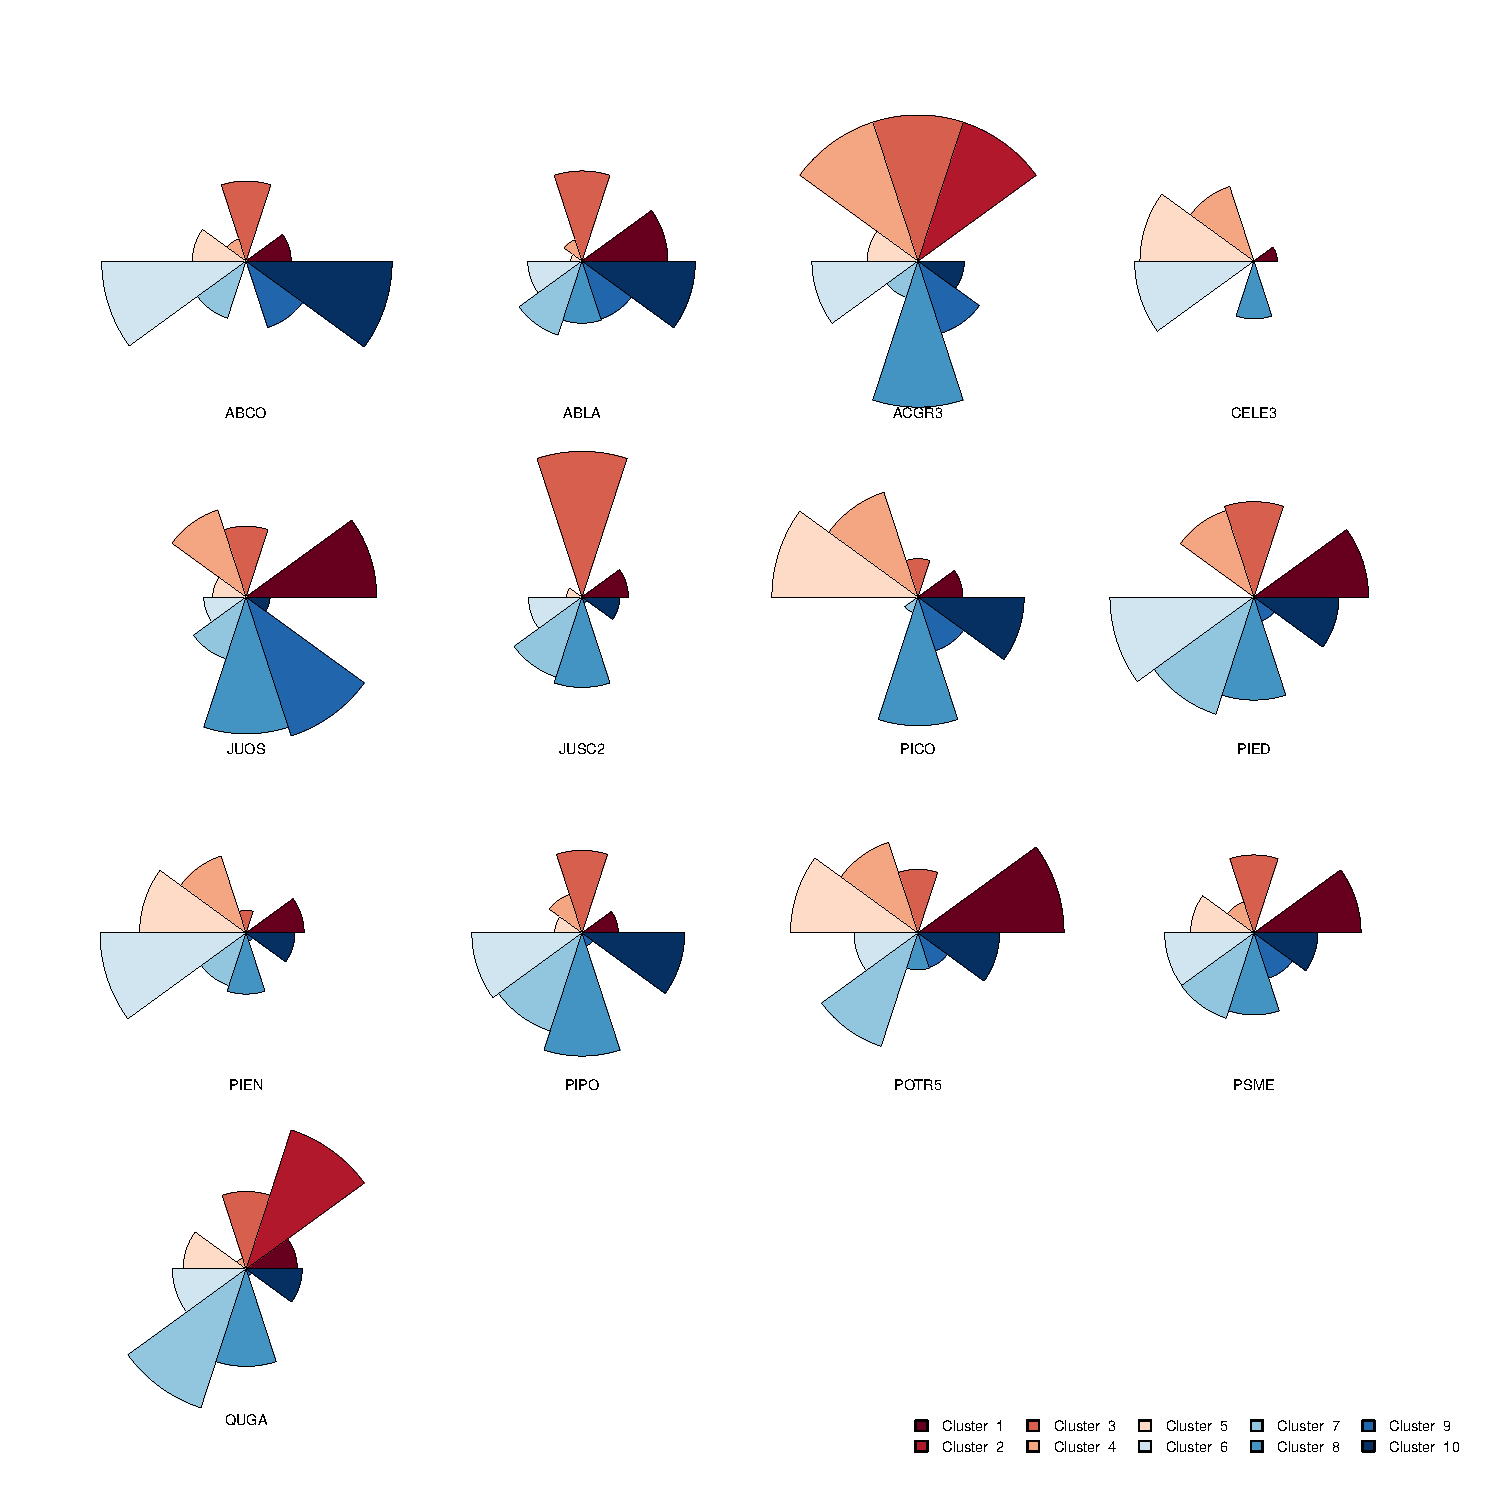
\includegraphics[width=12cm,height=8cm,keepaspectratio]{plot003.pdf}
  \caption{Cluster distribution across species.}
  \label{figure:fig003}
\end{figure}

In this type of graph each slice size is proportional to the probability
of belonging, and it is possible to note that some species of trees are
more or less associated with some clusters. For example, QUGA species is
more associated with Clusters 7 and 2 as well ACGR3 species.

\section{Conclusion.}\label{conclusion.}

The goal of this paper was describe the Bayesian LDA model for fuzzy
clustering based on different types of data, specifically we
demonstrated how to use the model for Multinomial entry in the Marketing
example, Binomial trial using the Landsat dataset and Bernoulli trial
using ecological data.

Also, we present the results in three different ways showing the
flexibility to use the results and represent the information numerically
and/or visually which is important when we faced large datasets and a
great number of possible clusters.

One of the main properties of the model presented here is the fact that
this model adopts the truncated stick-breaking prior which enables the
selection of the optimal number of clusters which regularizes model
results. The next step in the development of the model presented here is
the possibility to work with explanatory variables in the same structure
described in this article, which can be useful not only to model the
cluster but also explain how the clusters are created.

\section*{Appendix.}\label{appendix.}
\addcontentsline{toc}{section}{Appendix.}

Here in the Appendix we will show how the Full Conditional Distributions
were constructed. Consider initially the Full Conditional Distributions
for \(Z_{lc}=c^{*}\) in all three cases the kernel of the distribution
derived is the same:

\begin{equation*}
\begin{array}{lll}
p(Z_{lc}=c^{*}|Y_{ls}=s,\boldsymbol\zeta_{c^{*}},\boldsymbol\theta_{l})&=&\kappa\left[\phi_{c^{*}1}^{\mathbbm{1}(Y_{l1}=s,Z_{lc}=c^{*})}\times\dots\times \phi_{c^{*}S}^{\mathbbm{1}(Y_{lS}=s,Z_{lc}=c^{*})}\right]\\[.5em]
&&\times\left[\theta_{l1}^{\mathbbm{1}(Z_{l1}=c^{*})}\times\dots\times\theta_{lC}^{\mathbbm{1}(Z_{lC}=c^{*})}\right]\\[.5em]
&=&\kappa\zeta_{c^{*}s}\theta_{lc^{*}}
\end{array}
\label{ap:eq0001} 
\end{equation*}

\noindent where \(\mathbbm{1}(Y_{l1}=s,Z_{lc}=c^{*})\) is the indicator
function which assumes one only for the \(l\)-th observation, \(s\)-th
variable and has been identified as belong to cluster \(c^{*}\). In a
similar way, \(\mathbbm{1}(Z_{lC}=c^{*})\) assumes one only for
observations classified as belong to cluster \(c^{*}\).

Since \(Z_{lc}\) is a categorical random variable with support in
\(\Za=(1,2,\dots,C)\) the sum of all probabilities for all elements must
one, then the constant \(\kappa\) is given by:

\begin{equation*}
\begin{array}{lll}
\kappa&=&\left(\theta_{l1}\zeta_{1s}+\dots+\theta_{lC}\zeta_{Cs}\right)^{-1}
\end{array}
\label{ap:eq0002} 
\end{equation*}

Then, each category for \(Z_{lc}\) can be draw from a categorical
distribution with probabilities equal to
\(\kappa\zeta_{c^{*}s}\theta_{lc^{*}}\) with \(c^{*} \in \Za\), where
\(\zeta_{c^{*}s}=\phi_{sc^{*}}\) in the multinomial case and
\(\zeta_{c^{*}s}=\phi_{c^{*}s}^{y_{ls}}(1-\phi_{c^{*}s})^{1-y_{ls}}\)
and
\(\zeta_{c^{*}s}=\phi_{c^{*}s}^{x_{ils}}(1-\phi_{c^{*}s})^{1-x_{ils}}\)
for Bernoulli and Binomial cases respectively.

For the Bernoulli and Binomial cases, we have, respectively.:

\begin{equation*}
\begin{array}{lll}
p(Z_{lc}=c^{*}|Y_{ls}=s,\boldsymbol\phi_{c^{*}},\boldsymbol\theta_{l})&\propto&\theta_{lc^{*}}\phi_{c^{*}s}^{y_{ls}}(1-\phi_{c^{*}s})^{1-y_{ls}}
\end{array}
\label{ap:eq0003} 
\end{equation*}

\begin{equation*}
\begin{array}{lll}
p(Z_{lc}=c^{*}|Y_{ls}=s,\boldsymbol\phi_{c^{*}},\boldsymbol\theta_{l})&\propto&\theta_{lc^{*}}\phi_{c^{*}s}^{x_{ils}}(1-\phi_{c^{*}s})^{1-x_{ils}}
\end{array}
\label{ap:eq0004} 
\end{equation*}

\noindent where each cluster label can be draw from a categorical
distribution with probabilities equal to (Multinomial, Bernoulli and
Binomial):

\begin{equation*}
\begin{array}{lll}
p(Z_{lc}=c^{*}|Y_{ls}=s,\boldsymbol\phi_{c^{*}},\boldsymbol\theta_{l})&=&\frac{\theta_{lc^{*}}\phi_{c^{*}s}}{\displaystyle\sum_{c=1}^{C}\theta_{lc}\phi_{cs}}
\end{array}
\label{ap:eq0005} 
\end{equation*}

\begin{equation*}
\begin{array}{lll}
p(Z_{lc}=c^{*}|Y_{ls}=s,\boldsymbol\phi_{c^{*}},\boldsymbol\theta_{l})&=&\frac{\theta_{lc^{*}}\phi_{c^{*}s}^{y_{ls}}(1-\phi_{c^{*}s})^{1-y_{ls}}}{\displaystyle\sum_{c=1}^{C}\theta_{lc}\phi_{cs}^{y_{ls}}(1-\phi_{cs})^{1-y_{ls}}}
\end{array}
\label{ap:eq0006} 
\end{equation*}

\begin{equation*}
\begin{array}{lll}
p(Z_{lc}=c^{*}|Y_{ls}=s,\boldsymbol\phi_{c^{*}},\boldsymbol\theta_{l})&=&\frac{\theta_{lc^{*}}\phi_{c^{*}s}^{x_{ils}}(1-\phi_{c^{*}s})^{1-x_{ils}}}{\displaystyle\sum_{c=1}^{C}\theta_{lc}\phi_{cs}^{x_{ils}}(1-\phi_{cs})^{1-x_{ils}}}
\end{array}
\label{ap:eq0007} 
\end{equation*}

For the \(\boldsymbol\phi_{c^{*}}\) its Full Conditional is given by:

\begin{equation*}
\begin{array}{lll}
p\left(\boldsymbol\phi_{c^{*}}|\mathbf{Z}_{\cdot c^{*}},\{\mathbf{Y}_{l\cdot}|Z_{lc}=c^{*}\},\boldsymbol\beta\right)&\propto& \displaystyle\prod_{l=1}^{L}\phi_{c^{*}1}^{\mathbbm{1}(Y_{l1}=1,Z_{lc}=c^{*})}\times\dots\times\phi_{c^{*}S}^{\mathbbm{1}(Y_{l1}=S,Z_{lc}=c^{*})}\\[.5em]
&\times&\phi_{c^{*}1}^{\beta_{1}-1}\times\dots\times\phi_{c^{*}S}^{\beta_{S}-1}\\[.5em]
&\propto&\displaystyle\prod_{s=1}^{S}\phi_{c^{*}s}^{n_{c^{*}s}+\beta_{s}-1}
\end{array}
\label{ap:eq0005} 
\end{equation*}

\noindent where \(n_{c^{*}s}\) is the total number of elements
classified in community \(c^{*}\) and independent variable \(s\). In the
Binomial or Bernoulli case the Full Conditional is given by:

\begin{equation*}
\begin{array}{lll}
p\left(\phi_{c^{*}s}|\mathbf{Z}_{\cdot c^{*}},\{\mathbf{Y}_{l\cdot}|Z_{lc}=c^{*}\},\boldsymbol\beta\right)&\propto&\displaystyle\prod_{l=1}^{L}\phi_{c^{*}s}^{\mathbbm{1}(Y_{ls}=s,Z_{lc}=c^{*})}\phi_{c^{*}s}^{\alpha_{0}-1}(1-\phi_{c^{*}s})^{\alpha_{1}-1}\\[.5em]
&\propto&\phi_{c^{*}s}^{n_{c^{*}s}+\alpha_{0}-1}(1-\phi_{c^{*}s})^{n_{-c^{*}s}+\alpha_{1}-1}
\end{array}
\label{ap:eq0006} 
\end{equation*}

\noindent where \(n_{-c^{*}s}\) is the total number of elements that
\textbf{not} belong to either community \(c^{*}\) and independent
variable \(s\).

The last Full Conditional described here is the Full Conditional for
\(p\left(V_{lc}|Z_{lc}\right)\), in this case we have:

\begin{equation*}
\begin{array}{lll}
p\left(V_{lc}|Z_{lc}\right)&\propto& Binom(n_{lc}|N=N_{lc}+N_{l(c>c^{*})},V_{lc})Beta(V_{lc}|1,\gamma)\\[.5em]
&\propto&Beta(1+N_{lc},\gamma+N_{l(c>c^{*})})\\[.5em]
&=&\frac{\Gamma(N_{lc}+1+N_{l(c>c^{*})}+\gamma)}{\Gamma(N_{lc}+1)\Gamma(N_{l(c>c^{*})}+\gamma)}V_{lc}^{N_{lc}}\left(1-V_{lc}^{N_{l(c>c^{*})}+\gamma}\right)
\end{array}
\label{ap:eq0007} 
\end{equation*}

\begin{sidewaysfigure}[ht]
    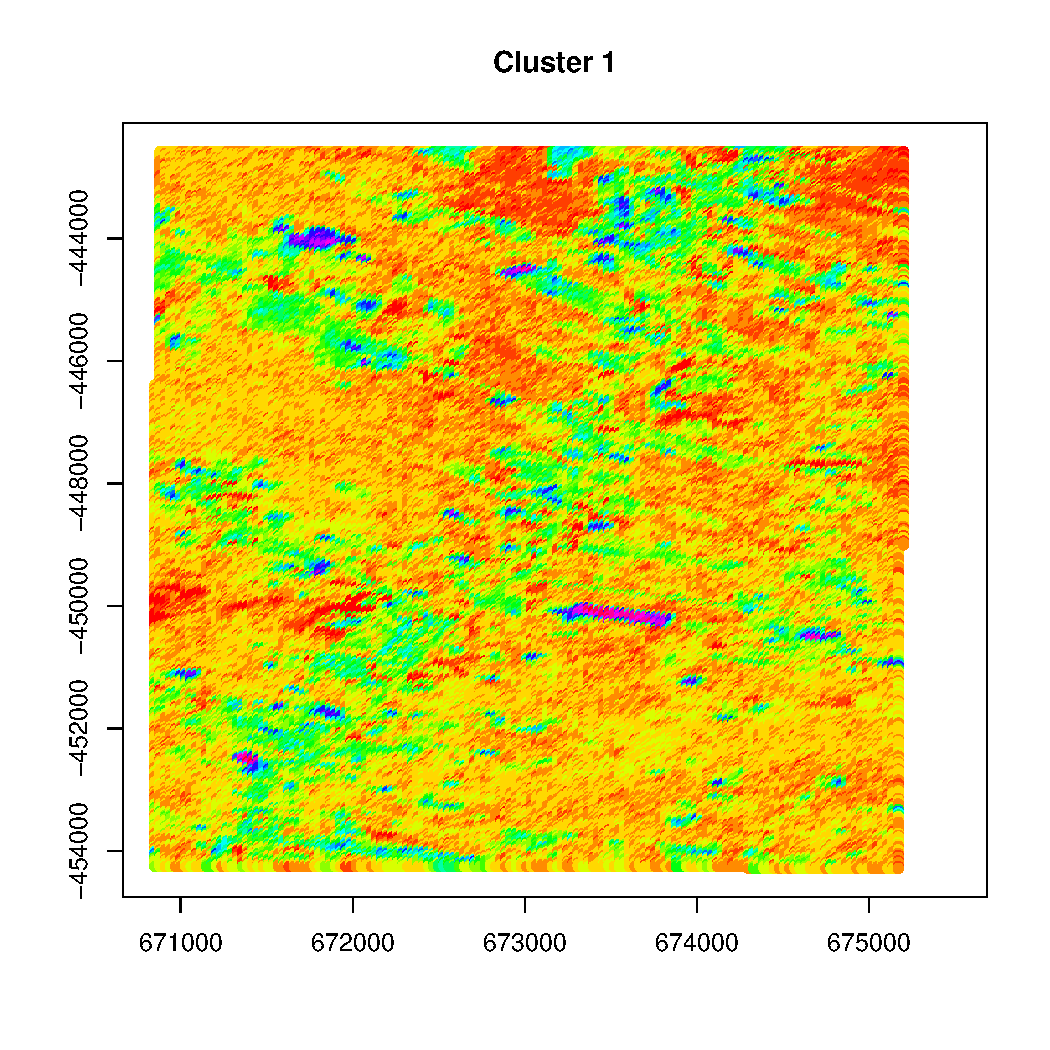
\includegraphics[width=\linewidth, height=0.85\textheight]{plot0021.pdf}
    \caption{Clusters 1 - Iquitos-Nauta road.}
    \label{figure:cluster1}
\end{sidewaysfigure}

\begin{sidewaysfigure}[ht]
    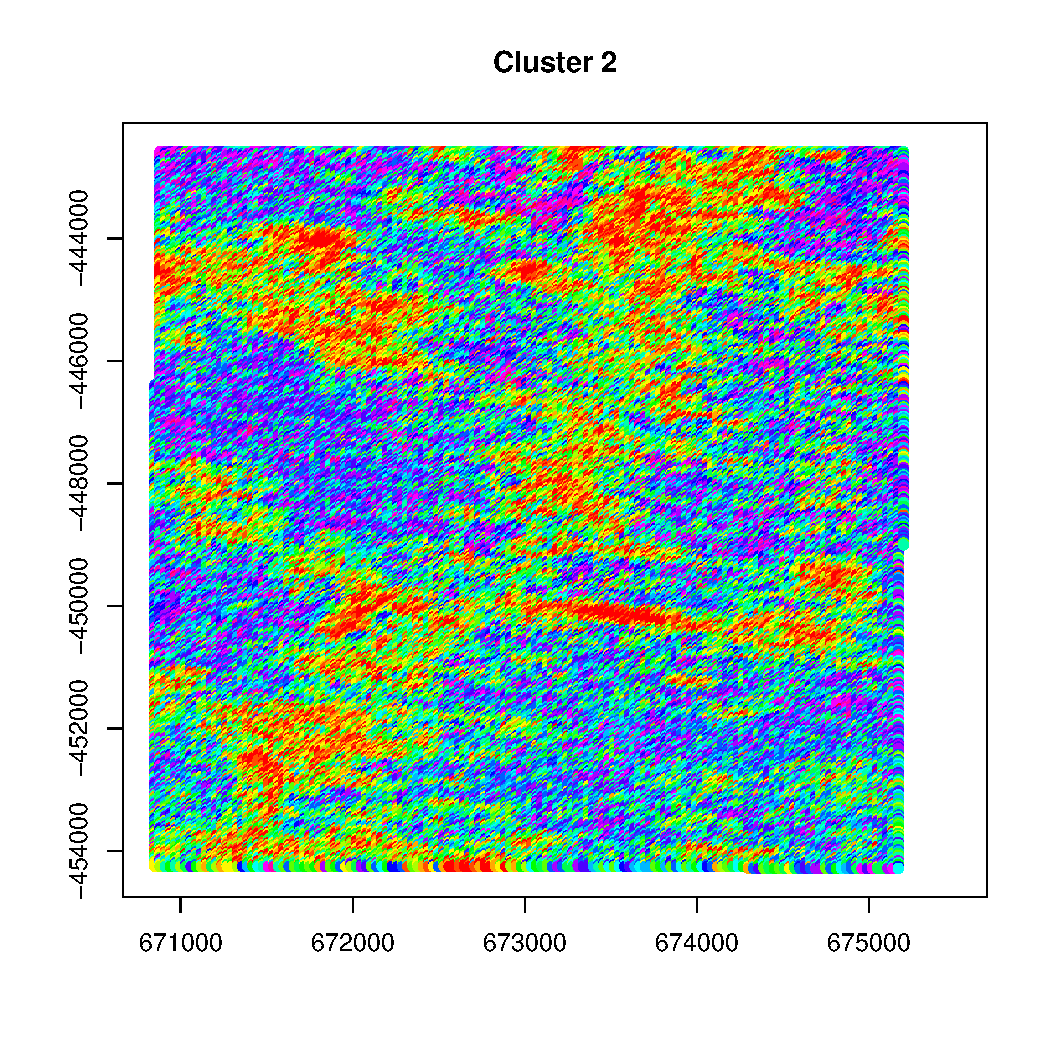
\includegraphics[width=\linewidth, height=0.85\textheight]{plot0022.pdf}
    \caption{Clusters 2 - Iquitos-Nauta road.}
    \label{figure:cluster2}
\end{sidewaysfigure}

\begin{sidewaysfigure}[ht]
    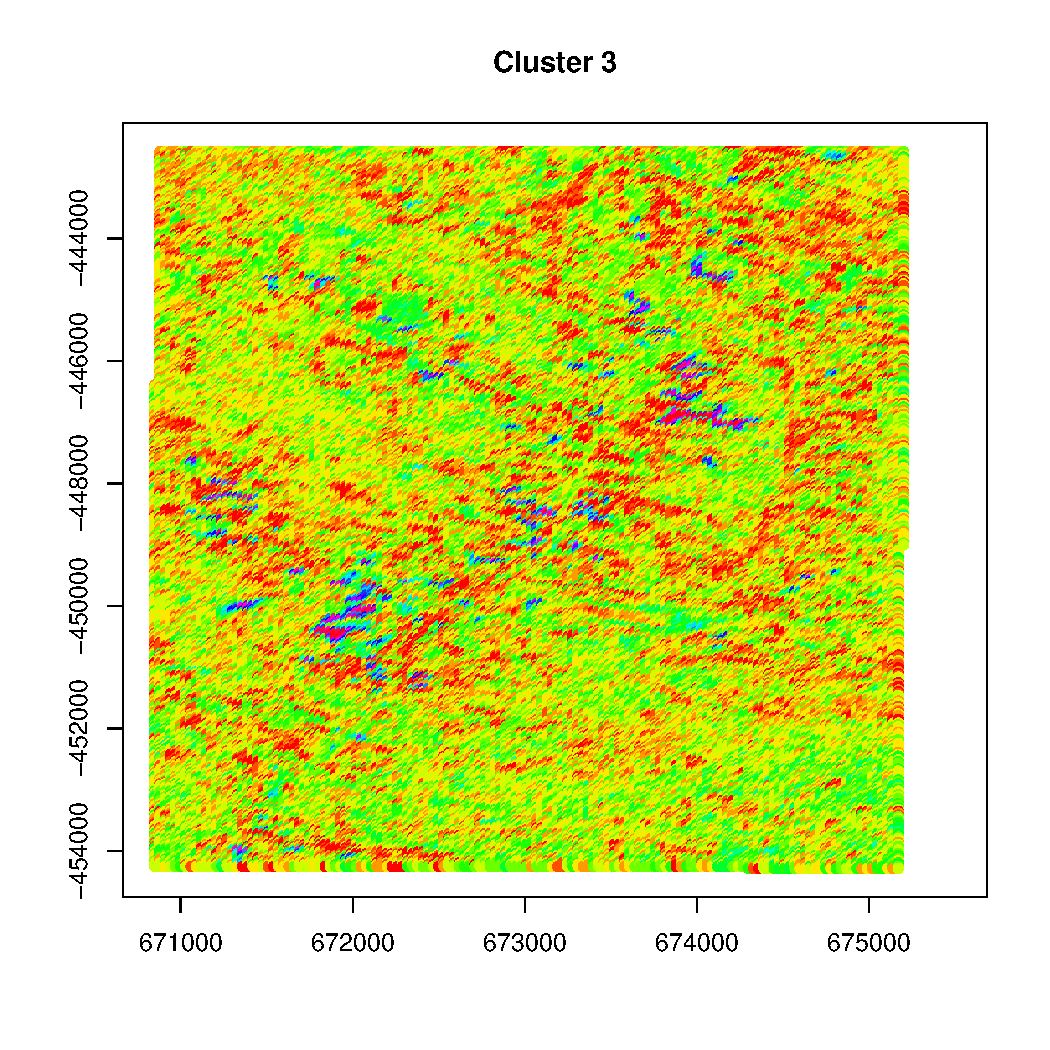
\includegraphics[width=\linewidth, height=0.85\textheight]{plot0023.pdf}
    \caption{Clusters 3 - Iquitos-Nauta road.}
    \label{figure:cluster3}
\end{sidewaysfigure}

\begin{sidewaysfigure}[ht]
    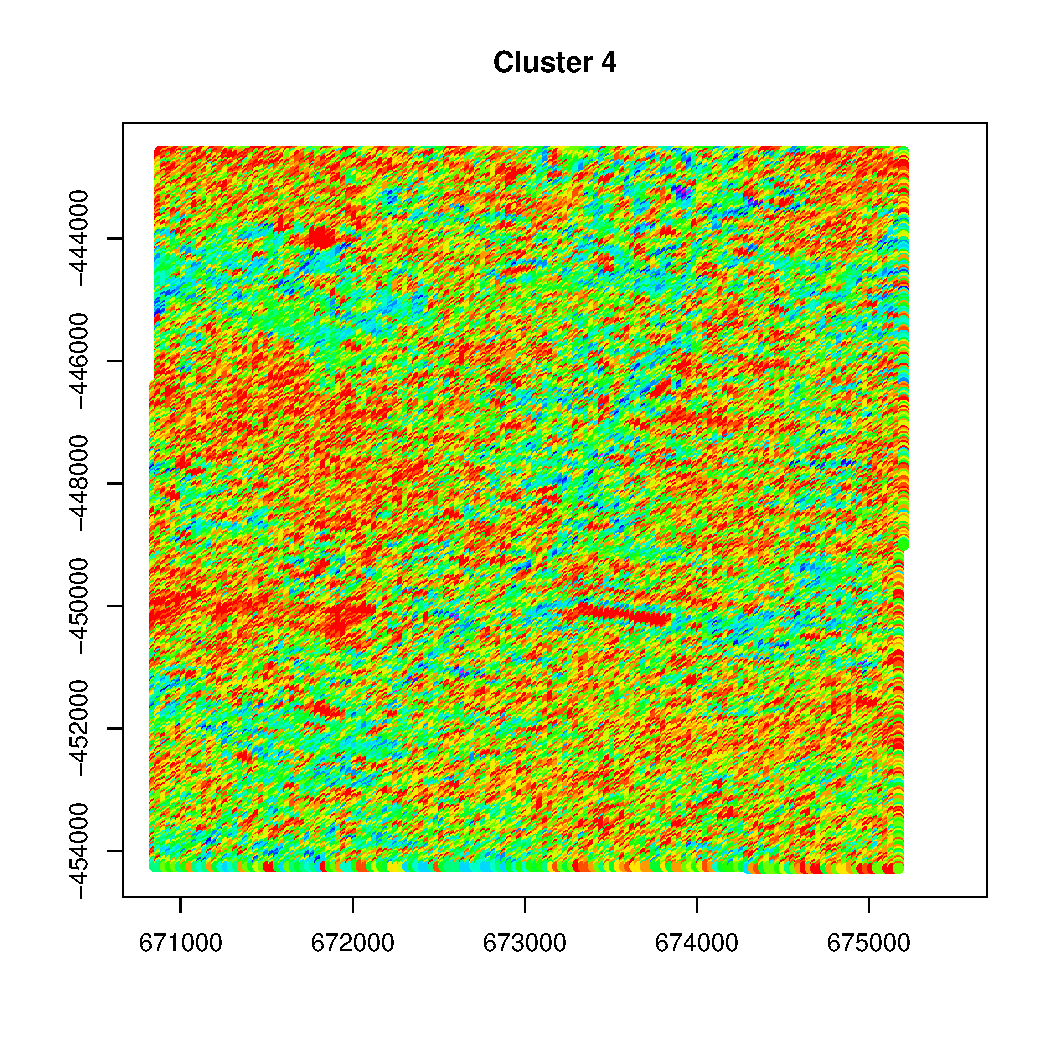
\includegraphics[width=\linewidth, height=0.85\textheight]{plot0024.pdf}
    \caption{Clusters 4 - Iquitos-Nauta road.}
    \label{figure:cluster4}
\end{sidewaysfigure}

\begin{sidewaysfigure}[ht]
    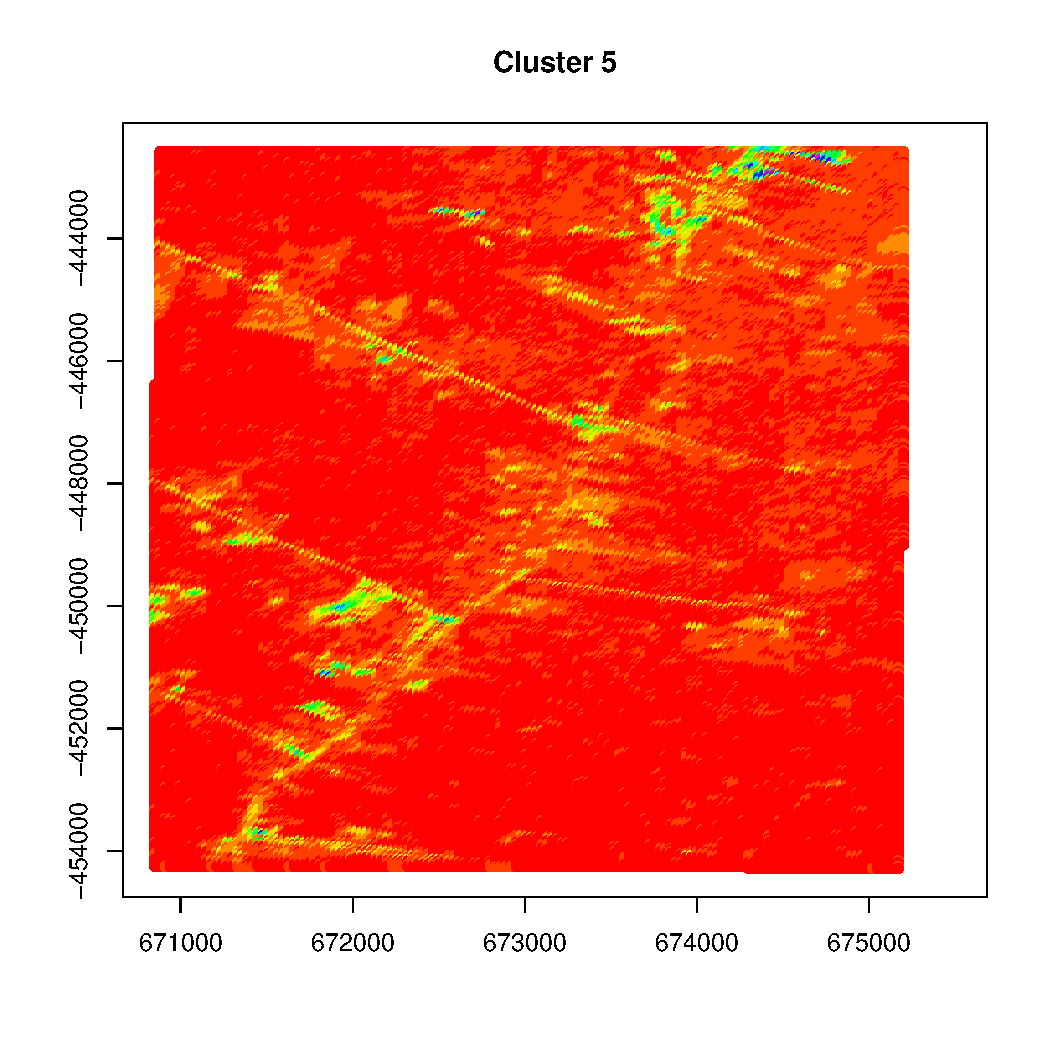
\includegraphics[width=\linewidth, height=0.85\textheight]{plot0025.pdf}
    \caption{Clusters 5 - Iquitos-Nauta road.}
    \label{figure:cluster5}
\end{sidewaysfigure}

\section*{References.}\label{references.}
\addcontentsline{toc}{section}{References.}

\hypertarget{refs}{}
\hypertarget{ref-airoldi2008mixed}{}
Airoldi, Edoardo M, David M Blei, Stephen E Fienberg, and Eric P Xing.
2008. ``Mixed Membership Stochastic Blockmodels.'' \emph{Journal of
Machine Learning Research} 9 (Sep): 1981--2014.

\hypertarget{ref-blei2003modeling}{}
Blei, David M, and Michael I Jordan. 2003. ``Modeling Annotated Data.''
In \emph{Proceedings of the 26th Annual International Acm Sigir
Conference on Research and Development in Informaion Retrieval},
127--34. ACM.

\hypertarget{ref-blei2003latent}{}
Blei, David M, Andrew Y Ng, and Michael I Jordan. 2003. ``Latent
Dirichlet Allocation.'' \emph{Journal of Machine Learning Research} 3
(Jan): 993--1022.

\hypertarget{ref-chang2012lda}{}
Chang, Jonathan. 2012. ``Lda: Collapsed Gibbs Sampling Methods for Topic
Models. R Package Version 1.4.2.''

\hypertarget{ref-griffiths2004finding}{}
Griffiths, Thomas L, and Mark Steyvers. 2004. ``Finding Scientific
Topics.'' \emph{Proceedings of the National Academy of Sciences} 101
(suppl 1). National Acad Sciences: 5228--35.

\hypertarget{ref-hornik2011topicmodels}{}
Hornik, Kurt, and Bettina Grün. 2011. ``Topicmodels: An R Package for
Fitting Topic Models.'' \emph{Journal of Statistical Software} 40 (13).
American Statistical Association: 1--30.

\hypertarget{ref-jones2016}{}
Jones, Thomas W. 2016. ``TextmineR: Functions for Text Mining and Topic
Modeling. R Package Version 2.0.2.''

\hypertarget{ref-keshava2003survey}{}
Keshava, Nirmal. 2003. ``A Survey of Spectral Unmixing Algorithms.''
\emph{Lincoln Laboratory Journal} 14 (1). LINCOLN LABORATORY M IT:
55--78.

\hypertarget{ref-kotler2006principles}{}
Kotler, Philip, and Gary Armstrong. 2006. ``Principles of Marketing
Management.'' Englewood Cliffs, NJ: Pearson Prentice-Hall.

\hypertarget{ref-lee2010empirical}{}
Lee, Sangno, Jeff Baker, Jaeki Song, and James C Wetherbe. 2010. ``An
Empirical Comparison of Four Text Mining Methods.'' In \emph{System
Sciences (Hicss), 2010 43rd Hawaii International Conference on}, 1--10.
IEEE.

\hypertarget{ref-lienou2010semantic}{}
Lienou, Marie, Henri Maître, and Mihai Datcu. 2010. ``Semantic
Annotation of Satellite Images Using Latent Dirichlet Allocation.''
\emph{IEEE Geoscience and Remote Sensing Letters} 7 (1). IEEE: 28--32.

\hypertarget{ref-mahajan2008mining}{}
Mahajan, Anuj, Lipika Dey, and Sk Mirajul Haque. 2008. ``Mining
Financial News for Major Events and Their Impacts on the Market.'' In
\emph{Web Intelligence and Intelligent Agent Technology, 2008.
Wi-Iat'08. Ieee/Wic/Acm International Conference on}, 1:423--26. IEEE.

\hypertarget{ref-mcauliffe2008supervised}{}
Mcauliffe, Jon D, and David M Blei. 2008. ``Supervised Topic Models.''
In \emph{Advances in Neural Information Processing Systems}, 121--28.

\hypertarget{ref-moisen2006predicting}{}
Moisen, Gretchen G, Elizabeth A Freeman, Jock A Blackard, Tracey S
Frescino, Niklaus E Zimmermann, and Thomas C Edwards. 2006. ``Predicting
Tree Species Presence and Basal Area in Utah: A Comparison of Stochastic
Gradient Boosting, Generalized Additive Models, and Tree-Based
Methods.'' \emph{Ecological Modelling} 199 (2). Elsevier: 176--87.

\hypertarget{ref-pearce2006modelling}{}
Pearce, Jennie L, and Mark S Boyce. 2006. ``Modelling Distribution and
Abundance with Presence-Only Data.'' \emph{Journal of Applied Ecology}
43 (3). Wiley Online Library: 405--12.

\hypertarget{ref-phan2013gibbslda}{}
Phan, Xuan-Hieu, and Cam-Tu Nguyen. 2013. ``GibbsLDA++, Ac/C++
Implementation of Latent Dirichlet Allocation (Lda) Using Gibbs Sampling
for Parameter Estimation and Inference.''

\hypertarget{ref-pritchard2000inference}{}
Pritchard, Jonathan K, Matthew Stephens, and Peter Donnelly. 2000.
``Inference of Population Structure Using Multilocus Genotype Data.''
\emph{Genetics} 155 (2). Genetics Soc America: 945--59.

\hypertarget{ref-roberts2014stm}{}
Roberts, Margaret E, Brandon M Stewart, and Dustin Tingley. 2014. ``Stm:
R Package for Structural Topic Models.'' \emph{R Package} 1: 12.

\hypertarget{ref-tirunillai2014mining}{}
Tirunillai, Seshadri, and Gerard J Tellis. 2014. ``Mining Marketing
Meaning from Online Chatter: Strategic Brand Analysis of Big Data Using
Latent Dirichlet Allocation.'' \emph{Journal of Marketing Research} 51
(4). American Marketing Association: 463--79.

\hypertarget{ref-tsai2011tag}{}
Tsai, Flora S. 2011. ``A Tag-Topic Model for Blog Mining.'' \emph{Expert
Systems with Applications} 38 (5). Elsevier: 5330--5.

\hypertarget{ref-dennis}{}
Tucker-Lima, Vittor, J. n.d. ``Does Deforestation Promote or Inhibit
Malaria Transmission in the Amazon? A Systematic Literature Review and
Critical Appraisal of Current Evidence.'' \emph{Philosophical
Transaction of the Royal Society B: Biological Sciences. In Press.}

\hypertarget{ref-valle2014decomposing}{}
Valle, Denis, Benjamin Baiser, Christopher W Woodall, and Robin Chazdon.
2014. ``Decomposing Biodiversity Data Using the Latent Dirichlet
Allocation Model, a Probabilistic Multivariate Statistical Method.''
\emph{Ecology Letters} 17 (12). Wiley Online Library: 1591--1601.

\hypertarget{ref-westgate2015text}{}
Westgate, Martin J, Philip S Barton, Jennifer C Pierson, and David B
Lindenmayer. 2015. ``Text Analysis Tools for Identification of Emerging
Topics and Research Gaps in Conservation Science.'' \emph{Conservation
Biology} 29 (6). Wiley Online Library: 1606--14.



\end{document}

